\section{Number Representation}

\begin{itemize}
    \item Numbers are represented in binary form in computers.
    \item Mathematical laws do not necessarily hold in computer arithmetic.
          (e.g. $3.14 + 1e20 - 1e20 \neq 3.14 + (1e20 - 1e20)$ due to precision and rounding errors)
    \item Numbers in computers are Finite Precision Numbers.
\end{itemize}

\begin{definition}[Finite Precision Numbers]\label{def:finite-precision-numbers}
    Finite Precision Numbers have the following characteristics:
    \begin{itemize}
        \item Limited number of bits to represent a number. (e.g. 32-bit integers)
        \item Limited range of numbers that can be represented. (e.g. $2^{32}$ for \texttt{unsigned int})
        \item Overflow and underflow occur when the number is too large or too small to be represented.
    \end{itemize}
\end{definition}

\subsection{Positional Number System and Radix}

\begin{definition}[Positional Number System]\label{def:positional-number-system}
    A positional number system is a system in which the position of a digit in a number determines
    its value. Numbers are represented in a string of digits in the form of:
    \begin{equation*}
        (a_na_{n-1}\ldots a_2a_1a_0.a_{-1}a_{-2}\ldots)_r
    \end{equation*}
    where:
    \begin{itemize}
        \item $n\in[0, +\infty)\cap \mathbb{Z}$,
        \item $r\in[2, +\infty)\cap\mathbb{Z}$ is the radix (base) of the number system,
              which determines the value of each digit at position $i$ as $r^i$,
        \item $a_i\in[0, r)$.
    \end{itemize}

    The value of the number being represented is given by:
    \begin{equation}\label{eq:positional-number-system-value-direct}
        \sum_{i} (a_i r^i) \quad\text{\bfseries (The Direct Approach)}
    \end{equation}
\end{definition}

Generally, the radix value is one of 2 (binary), 8 (octal), 10 (decimal), or 16 (hexadecimal).

\begin{example}
    The number 1A6.BE$_{16}$ is a fractional number in hexadecimal system. Its value in decimal system is:
    \begin{align*}
        \text{1A6.BE}_{16} &=
            1\times 16^2 + 10\times 16^1 + 6\times 16^0 + 11\times 16^{-1} + 14\times 16^{-2} \\
            &= 422.7421875_{10}
    \end{align*}
\end{example}

\begin{theorem}[Iterative Approach of Evaluating the Value of a Positional Number]
    The value of a number in a positional number system can be evaluated alternatively by:
    \begin{equation}\label{eq:positional-number-system-value-iterative}
        r\left(r\left(r\left(r\cdot a_n + a_{n-1}\right)+ a_{n-2}\right)+ a_{n-3} \dots\right) + a_0
        \quad \text{\bfseries (The Iterative Approach)}
    \end{equation}
    which is more efficient than the direct approach.
\end{theorem}

\begin{proof}
    Consider only the integer case.
    For the direct approach, for each digit $a_i$, its value is calculated by \[
        a_i \underbrace{\times r \times r \times \dots \times r}_{i\text{ times}}
    \] Therefore, for $i=n$, the number of multiplications performed is $n$ times.
    The total number of multiplications performed to convert a number of $n$ digits is \[
        1+2+3+\dots+n = \frac{n(n+1)}{2} = O(n^2)
    \]

    For the iterative approach, the left most digit ($a_n$) is first multiplied by $r$ and added to
    the next digit ($a_{n-1}$). This sum is then multiplied by $r$ and added to the next digit
    ($a_{n-2}$), and so on. The total number of multiplications performed is $n$ times. Therefore,
    the iterative approach has a linear complexity $O(n)$.

    Hence, the iterative approach is more efficient than the direct approach.
\end{proof}

\subsection{Integer Representation}

\subsubsection{Unsigned Integer Representation}

\begin{definition}
    For a sequence of $n$ bits ($a_{n-1}a_{n-2}\ldots a_1a_0$), it represents a nonnegative integer
    of value A, where
    \begin{equation*}
        A = \sum_{i=0}^{n-1} 2^i a_i
    \end{equation*}
\end{definition}

\subsubsection{Sign-and-Magnitude Representation}

\begin{definition}
    For a sequence of $n$ bits, the MSB\footnotemark is used
    to represent the sign of the number. The rest $n-1$ bits represent the magnitude of the number.
    The value of the number is given by:
    \begin{equation*}
        A = (-1)^{a_{n-1}} \sum_{i=0}^{n-2} 2^i a_i
    \end{equation*}

    \begin{example}
    For 4-bit integers, we have:
    \begin{align*}
        \boldsymbol{0}0110101_2 &= \boldsymbol{+}53_{10} \\
        \boldsymbol{1}0110101_2 &= \boldsymbol{-}53_{10}
    \end{align*}
    \end{example}

\end{definition}

\footnotetext{Most Significant Bit (the leftmost bit)}

This representation has two pitfalls:
\begin{enumerate*}
    \item It has two represtations for zero ($0000_2$) and ($1000_2$).
    \item It is inconvenient for arithmetic operations.
\end{enumerate*}
Therefore, this representation is rarely used to represent integers.

\subsubsection{One's and Two's Complement Representation}

\begin{definition}[One's Complement]
    For each positive integer, its one's complement representation is unchanged. For each negative
    number, its one's complement representation is obtained by flipping all the bits of its
    corresponding positive number.

    \begin{example}
        For 8-bit representation of $+8$, its one's complement is $0000\,1000_2$.
        For $-8$, its one's complement is obtained by flipping every bit of +8, which is $1111\,0111_2$.
    \end{example}
\end{definition}

One's Complement representation still has two representations for zero ($0000_2$) and ($1111_2$).
Therefore, Two's Complement representation is more commonly used.

\begin{definition}[Two's Complement]
    For each positive integer, its two's complement representation is unchanged. For each negative
    number, its two's complement representation is obtained by adding 1 to its one's complement.

    \begin{example}
        For 8-bit representation of $+13$, its two's complement is $0000\,1101_2$. For $-13$, its
        two's complement is obtained by adding 1 to its one's complement, which is
        $1111\,0010_2 + 0000\,0001_2 = 1111\,0011_2$.
    \end{example}

    \begin{equation*}
        A = -2^{n-1}a_{n-1} + \sum_{i=0}^{n-2} 2^i a_i
    \end{equation*}
\end{definition}

For the ``negative zero'', by the definition of two's complement, its 8-bit representation will be
$-0_{10} = 1111\,1111_2 + 0000\,0001_2 = 1\,0000\,0000_2$. However, since the result is 9 bits, the
carry bit is discarded, and the result is $0000\,0000_2$, which is the same as the representation of
the ``positive zero''. The two's complement has only one representation for zero.

For arithmetic operations, simply add the two numbers together, and discard any carry from the MSB,
the result will be the correct answer.

\begin{remark}
    Like the Sign-and-Magnitude representation, the One's and Two's Complement representations use
    the MSB as the sign bit.
\end{remark}

\begin{theorem}[Overflow Rule for Two's Complement]\label{thm:overflow-rule-twos-complement}
    When two numbers of the same sign are added, overflow occurs iff the result has an opposite sign.
\end{theorem}

\subsubsection{Range Extension}

It is sometimes useful to store an integer that requires $n$ bits in $m$ bits ($m>n$). Different
methods are needed for different representations.

\begin{itemize}
    \item \textbf{Unsigned Integer}: Add more bits to the left and fill them with zeros.
    \item \textbf{Sign-and-Magnitude}: Add more bits to the left. Move the sign bit to the new MSB,
            and fill the rest with zeros.
    \item \textbf{Two's Complement}: Add more bits to the left. Fill the new bits with the sign bit.
            (\textbf{Sign Extension})
\end{itemize}

\subsection{Integer Arithmetic Operations}

\subsubsection{Negation of Two's Complement}

\begin{definition}[Negation of Two's Complement]
To negate a number in Two's Complement representation, take the Two's Complement of the number.
\end{definition}

\subsubsection{Addition and Subtraction}

Addition of two numbers in Two's Complement is the same as if they were unsigned integers.
Refer to Theorem \ref{thm:overflow-rule-twos-complement} for overflow rule. For subtraction,
negate the second operand and perform addition.

\subsubsection{Multiplication}

To make explanations clear, we call the first operand the \textbf{multiplicand} and the second
operand the \textbf{multiplier}.

For \textbf{unsigned integers}, perform:
\begin{enumerate}
    \item For the $i$-th bit of the multiplier, if it is 1, shift the multiplicand left
        by $i$ bits and add it to the partial sum. ($a_i$ as in $a_na_{n-1}\ldots a_1a_0$)
    \item If the $i$-th bit of the multiplier is 0, do nothing.
    \item Return the partial sum as the result.
\end{enumerate}

For \textbf{two's complement integers with both operands being positive}, perform the same 
steps as for unsigned integers.
For \textbf{two $n$-bit two's complement integers with one or both operands being negative},
perform:
\begin{enumerate}
    \item For the $i$-th bit of the multiplier, where $i\in[0, n-1]$, if it is 1, shift the
        multiplicand left by $i$ bits, then sign-extend it to $2n$ bits, and add it to the 
        partial sum.
    \item For the MSB of the multiplier,
        \begin{itemize}
            \item If it is 1, take the two's complement of the multiplicand, sign-extend it
                to $2n$ bits, and add it to the partial sum.
            \item If it is 0, do nothing.
        \end{itemize}
    \item Sum the partial sums, ignore the carry bit, and return the result.
\end{enumerate}

\begin{example} [Multiplication of $-11$ and $-13$ in 8-bit two's complement]
    \begin{equation*}\begin{aligned}[t]\begin{arithmetic}[t]
                1111\,0011 &    (multiplicand $-13$) \\
        \times  1111\,0101 &    (multiplier $-11$)   \\
    1111\,1111\,1111\,0011 &    (left shift by 0, sign-extend) \\
    1111\,1111\,1100\,11~~ &    (left shift by 2, sign-extend) \\ 
    1111\,1111\,0011\,~~~~ &    $\cdots$ \\
    1111\,1110\,011~\,~~~~ \\
    1111\,1100\,11~~\,~~~~ \\
  + 0000\,0110\,1~~~\,~~~~ &    (two's complement of multiplicand, sign-extend) \\
    \cancel{101}\,0000\,0000\,1000\,1111 & (product $+143$)\\
    \end{arithmetic}\end{aligned}\end{equation*}
\end{example}

\begin{theorem}
    Multiplying an $n$-bit integer by an $m$-bit integer
    produces a product of at most $(n+m)$ bits.
\end{theorem}

\subsubsection{Division}

\textit{Not covered in this course.}

\subsection{Floating-Point Representation}

\subsubsection{Excess-$K$ (Bias) Representation}

\begin{definition}[Excess-$K$ Representation]
    In an $n$-bit Excess-$K$ representation, the values that are represented are in the interval of
    $[0 - K, 2^n - 1 - K]$, where the smallest value is represented by all bits being 0, and the
    greatest value is represented by all bits being 1.

    The $K$ is referred to an offset, or bias, as it is subtracted from the \textit{bit pattern value} to
    obtain the represented \textit{true value}.

    \begin{example}
        In a 3-bit Excess-5 representation, we have:

        \centering
        \begin{tabular}{|c|c|c|}
            \hline
            Bit Pattern & Bit Pattern Value & True Value \\
            \hline
            111 & 7 & 2 ($=7-5$) \\
            110 & 6 & 1 \\
            101 & 5 & 0 \\
            100 & 4 & -1 \\
            011 & 3 & -2 \\
            010 & 2 & -3 \\
            001 & 1 & -4 \\
            000 & 0 & -5 \\
            \hline
        \end{tabular}
    \end{example}

    The $K$ is typically chosen to be $2^{n-1}$ or $2^{n-1} - 1$, with the latter being more common.

    The Excess-$2^{n-1} - 1$ representation is used for representing a floating-point number
    as regulated by the IEEE\footnotemark standard.
\end{definition}

\footnotetext{Institute of Electrical and Electronics Engineers}

\subsubsection{IEEE 754-2008 Floating-Point Number Representation}

\begin{definition}[Format of a Floating-Point Number]
    A floating-point number is represented in the form of:
    \[\pm\,\text{Significand}\times 2^{\,\pm\,\text{(Biased) Exponent}}\]
\end{definition}

In a general 32-bit IEEE floating-point number, it is stored in memory by:

\begin{center}
    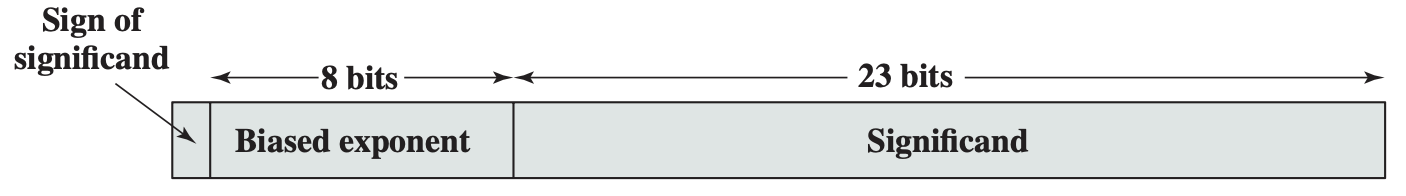
\includegraphics[scale=0.5]{chaps/number-representation/32-bit-ieee-float.png}
\end{center}

The floating-point number is always normalised before being stored. A normal number is the one
with the MSB being 1. The convention is to always make the radix point to the right of the MSB,
i.e. the MSB is always 1. Therefore, the MSB is never stored in memory. A normal nonzero number
takes the form:
\[\pm 1.\underbrace{\text{bbb}\ldots\text{b}}_{\text{23 bits}}\times 2^{\,\pm\,\text{E}}\]

The exponent is stored in Excess-$127$ ($2^{8-1} - 1$). Meaning that 127 is added to the true
exponent before being stored.

Note that since there is always a leading 1, the significand is always in the range of $[1, 2)$.
This implies that when the floating-point number is too far away from or too close to zero, it
cannot be represented accurately. The following diagram shows the range of representible values
of a 32-bit floating-point number (\textbf{not the IEEE standard}):

\begin{center}
    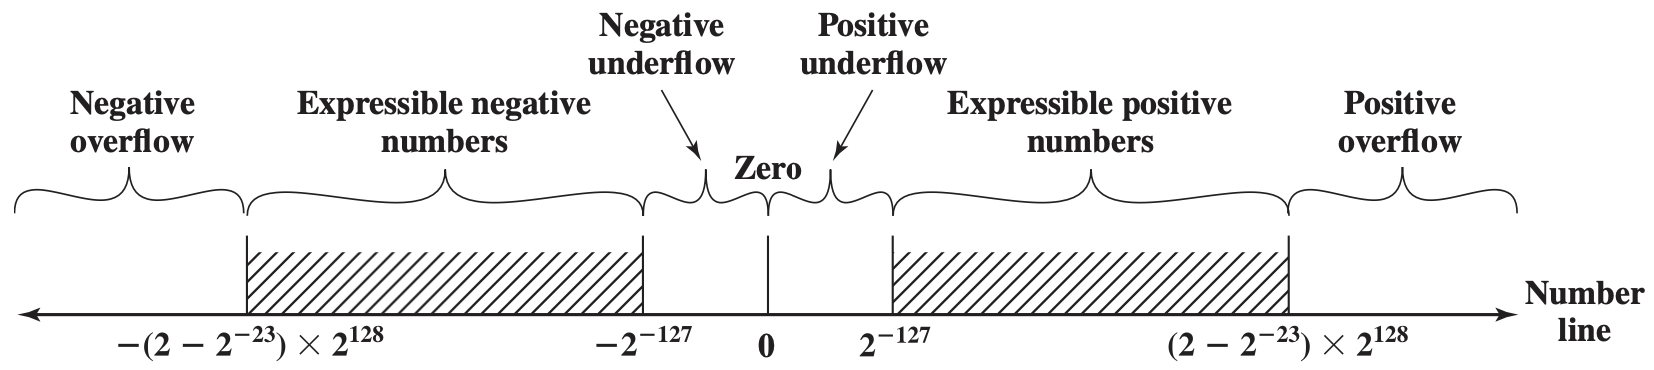
\includegraphics[scale=0.5]{chaps/number-representation/32-bit-ieee-float-range.png}
\end{center}

The diagram shows 0 is in the range of underflow, which can be inconvenient. Therefore, special
values are defined in the IEEE standard
to represent 0, $\pm\infty$, and \texttt{NaN} (Not a Number).
\begin{itemize}
    \item $\pm0$: Biased exponent and significand are all 0. The sign bit determines the sign.
    \item $\pm\infty$: Biased exponent is all 1, and significand is all 0.
    \item \texttt{NaN}: Biased exponent is all 1, and significand is not all 0.
    \item Subnormal numbers: Biased exponent is all 0, and significand is not all 0.
        ($\pm 2^{-126}(0.\text{S})$) Allows gradual underflow.
\end{itemize}

\begin{remark}
    In assignments and exams, unless specified, the above special meanings are not considered.
\end{remark}

IEEE 754-2008 defines three types of binary floating-point numbers - 
single precision (\texttt{Binary32}), double precision (\texttt{Binary64}), and
quadruple precision (\texttt{Binary128}). The following table shows the parameters of each type:

\begin{center}
    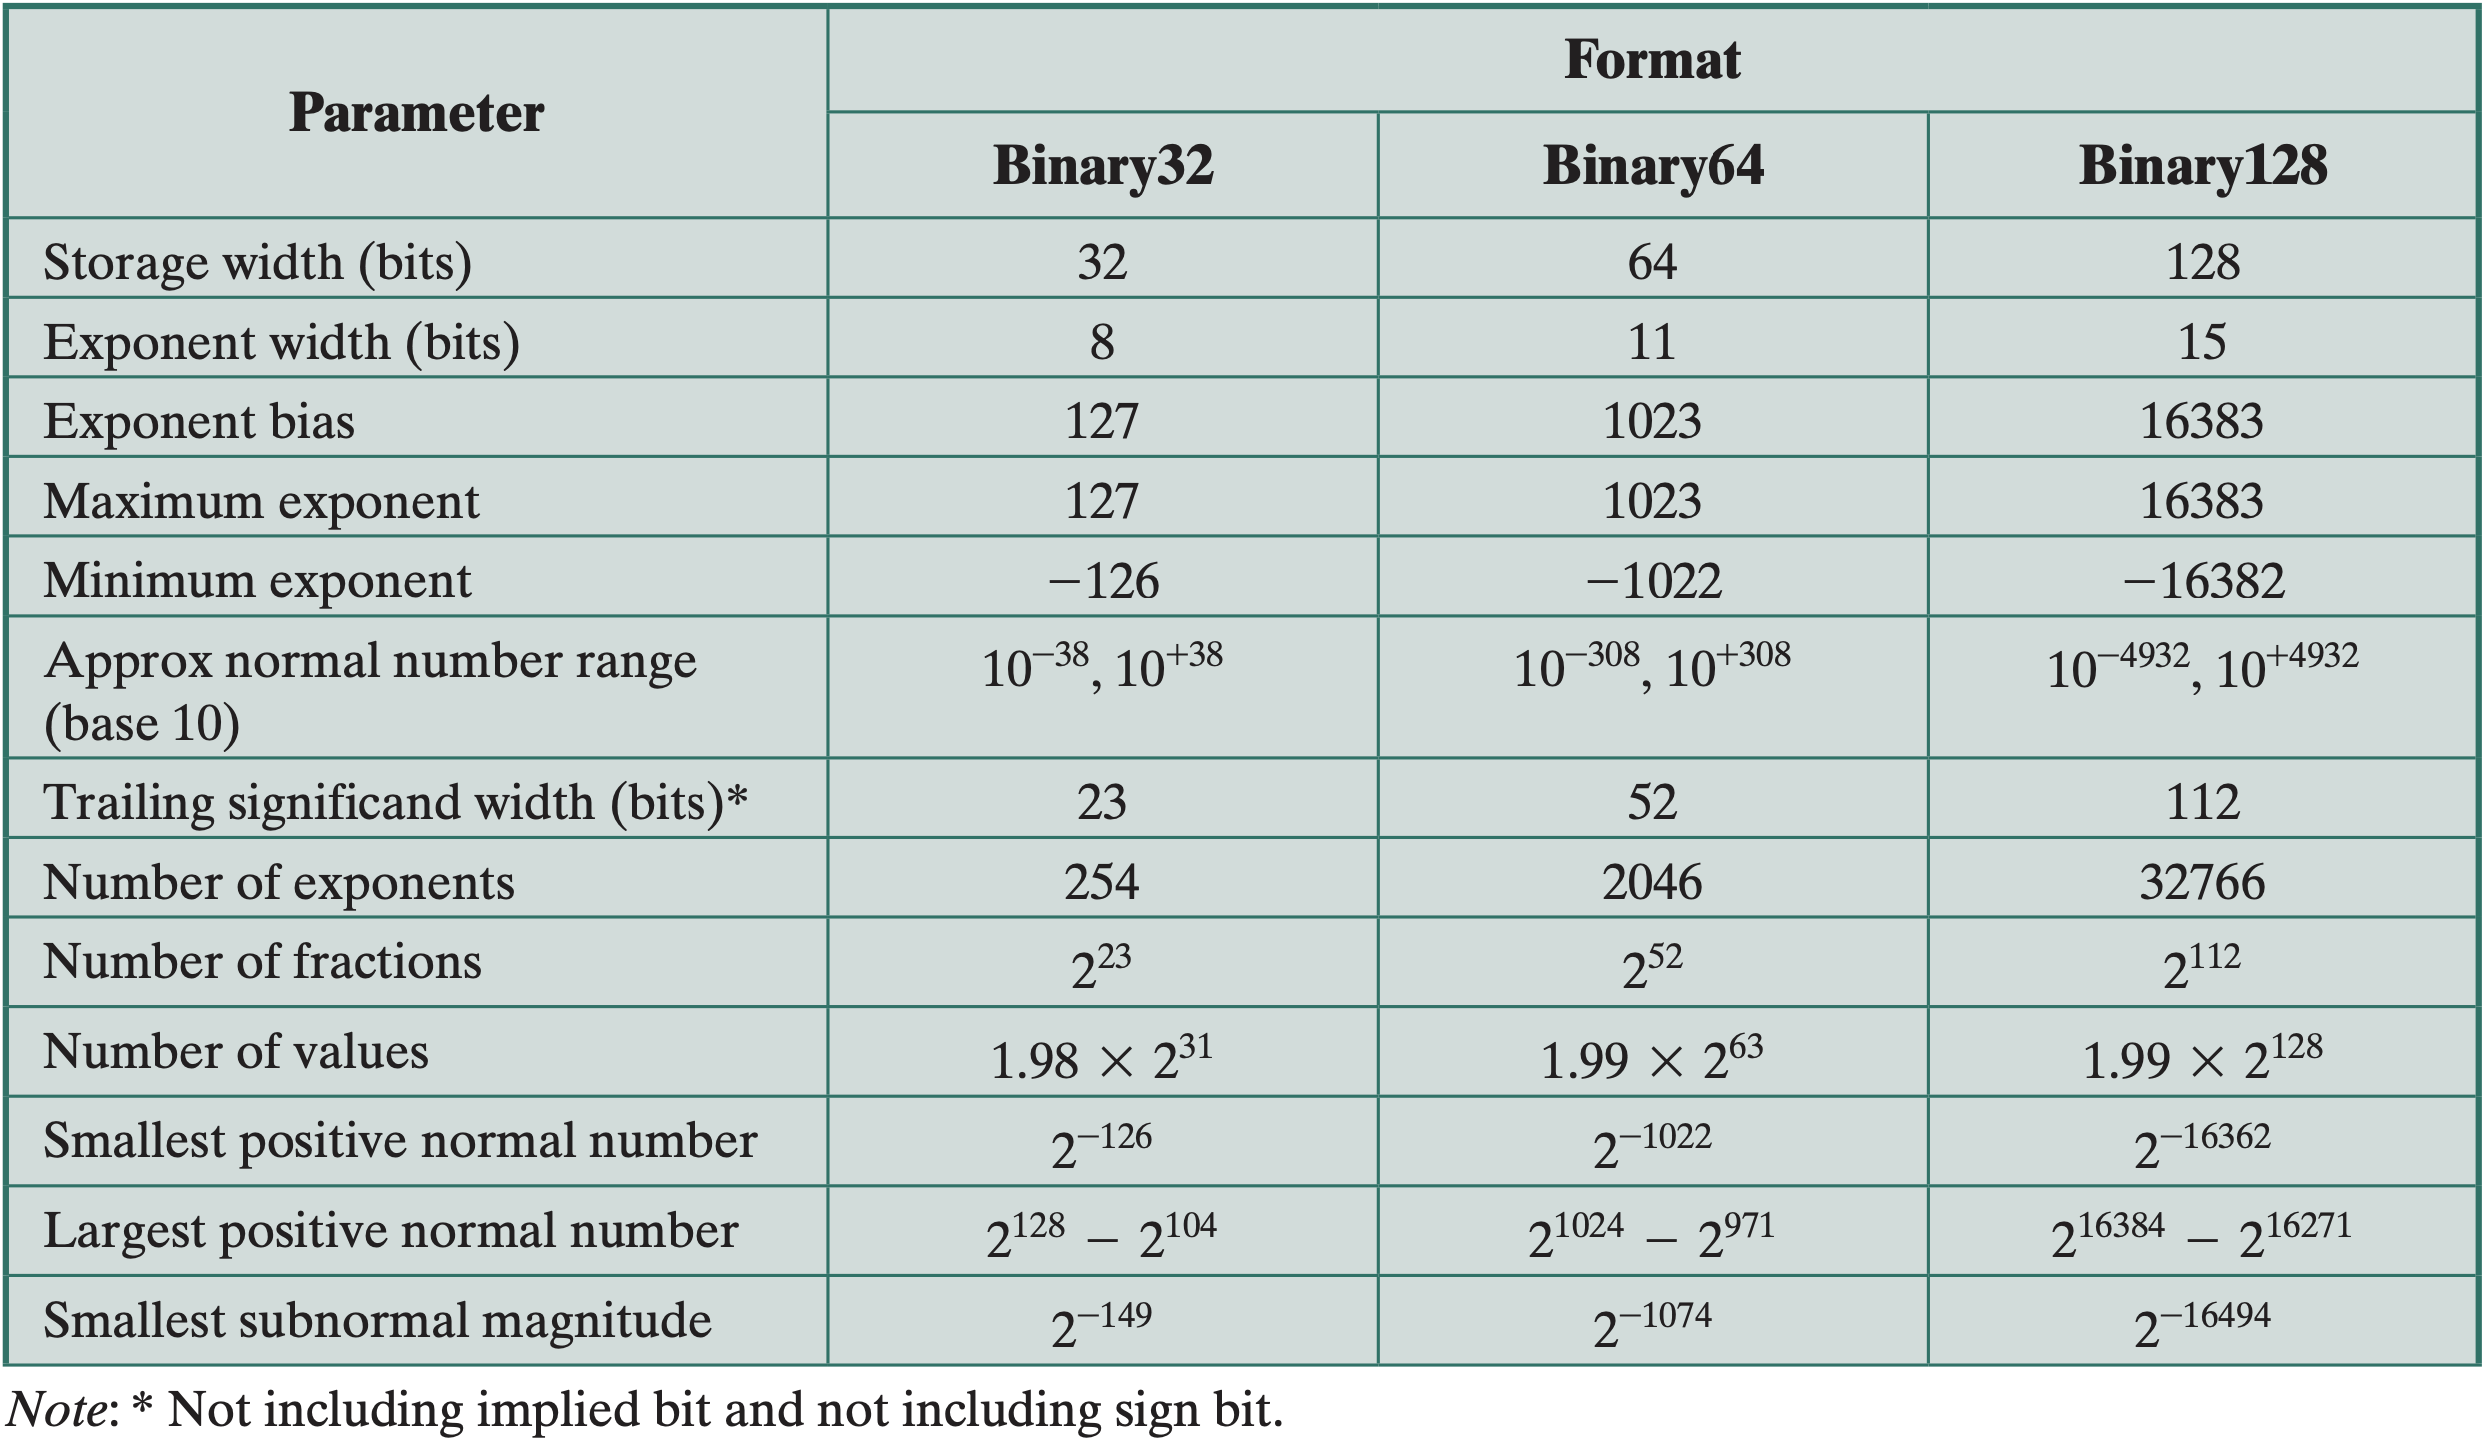
\includegraphics[scale=0.3]{chaps/number-representation/ieee-754-binary-float-parameters.png}
\end{center}

\begin{example}[Manual conversion of a decimal number to Binary32 floating-point number]
    To convert -23.875 to a 32-bit floating-point number, we have these steps:
    \begin{itemize}
        \item Convert -23.875 to binary: $-23.875_{10} = -10111.111_2$
        \item Normalise the binary number: $-10111.111_2 = -1.0111111_2\times 2^4$
        \item Convert the exponent to biased exponent: $4 + 127 = 131 = 10000011_2$
        \item Set the sign bit, biased exponent, and significand:
            $\boxed{\underbrace{1}_{\text{sign}}\,\underbrace{1000\,0011}_{\text{biased exponent}}\,
            \underbrace{0111\,1110\,0000\,0000\,0000\,000}_{\text{significand}}}$
    \end{itemize}
\end{example}

\begin{theorem}
    Some important properties of floating-point numbers:
    \begin{itemize}
        \item The number of representable values of a $n$-bit floating-point number is
            NOT greater than that of a $n$-bit integer (both being $2^n$).
        \item The representable values of a floating-point number are NOT uniformly distributed.
    \end{itemize}
\end{theorem}

\subsection{Floating-Point Arithmetic Operations}

\subsubsection{Addition and Subtraction}

Steps for floating-point number addition and subtraction:
\begin{enumerate}
    \item For the number with the smaller exponent, shift the significand right by the difference
        in the exponents to align their radix points.
    \item Add or subtract the significands, then determine the sign of the result.
    \item Normalise the result. Truncate the significand to the largest number of bits allowed.
\end{enumerate}

Generally, there are five phrases in floating-point addition and subtraction:
\begin{enumerate}
    \item \textbf{Check for zeros};
    \item \textbf{Alignment} of significands;
    \item \textbf{Addition/Subtraction} of significands;
    \item \textbf{Normalisation} of the result;
    \item \textbf{Rounding}.
\end{enumerate}

A typical floating-point addition/subtraction is illustrated in the following flowchart:

\begin{center}
    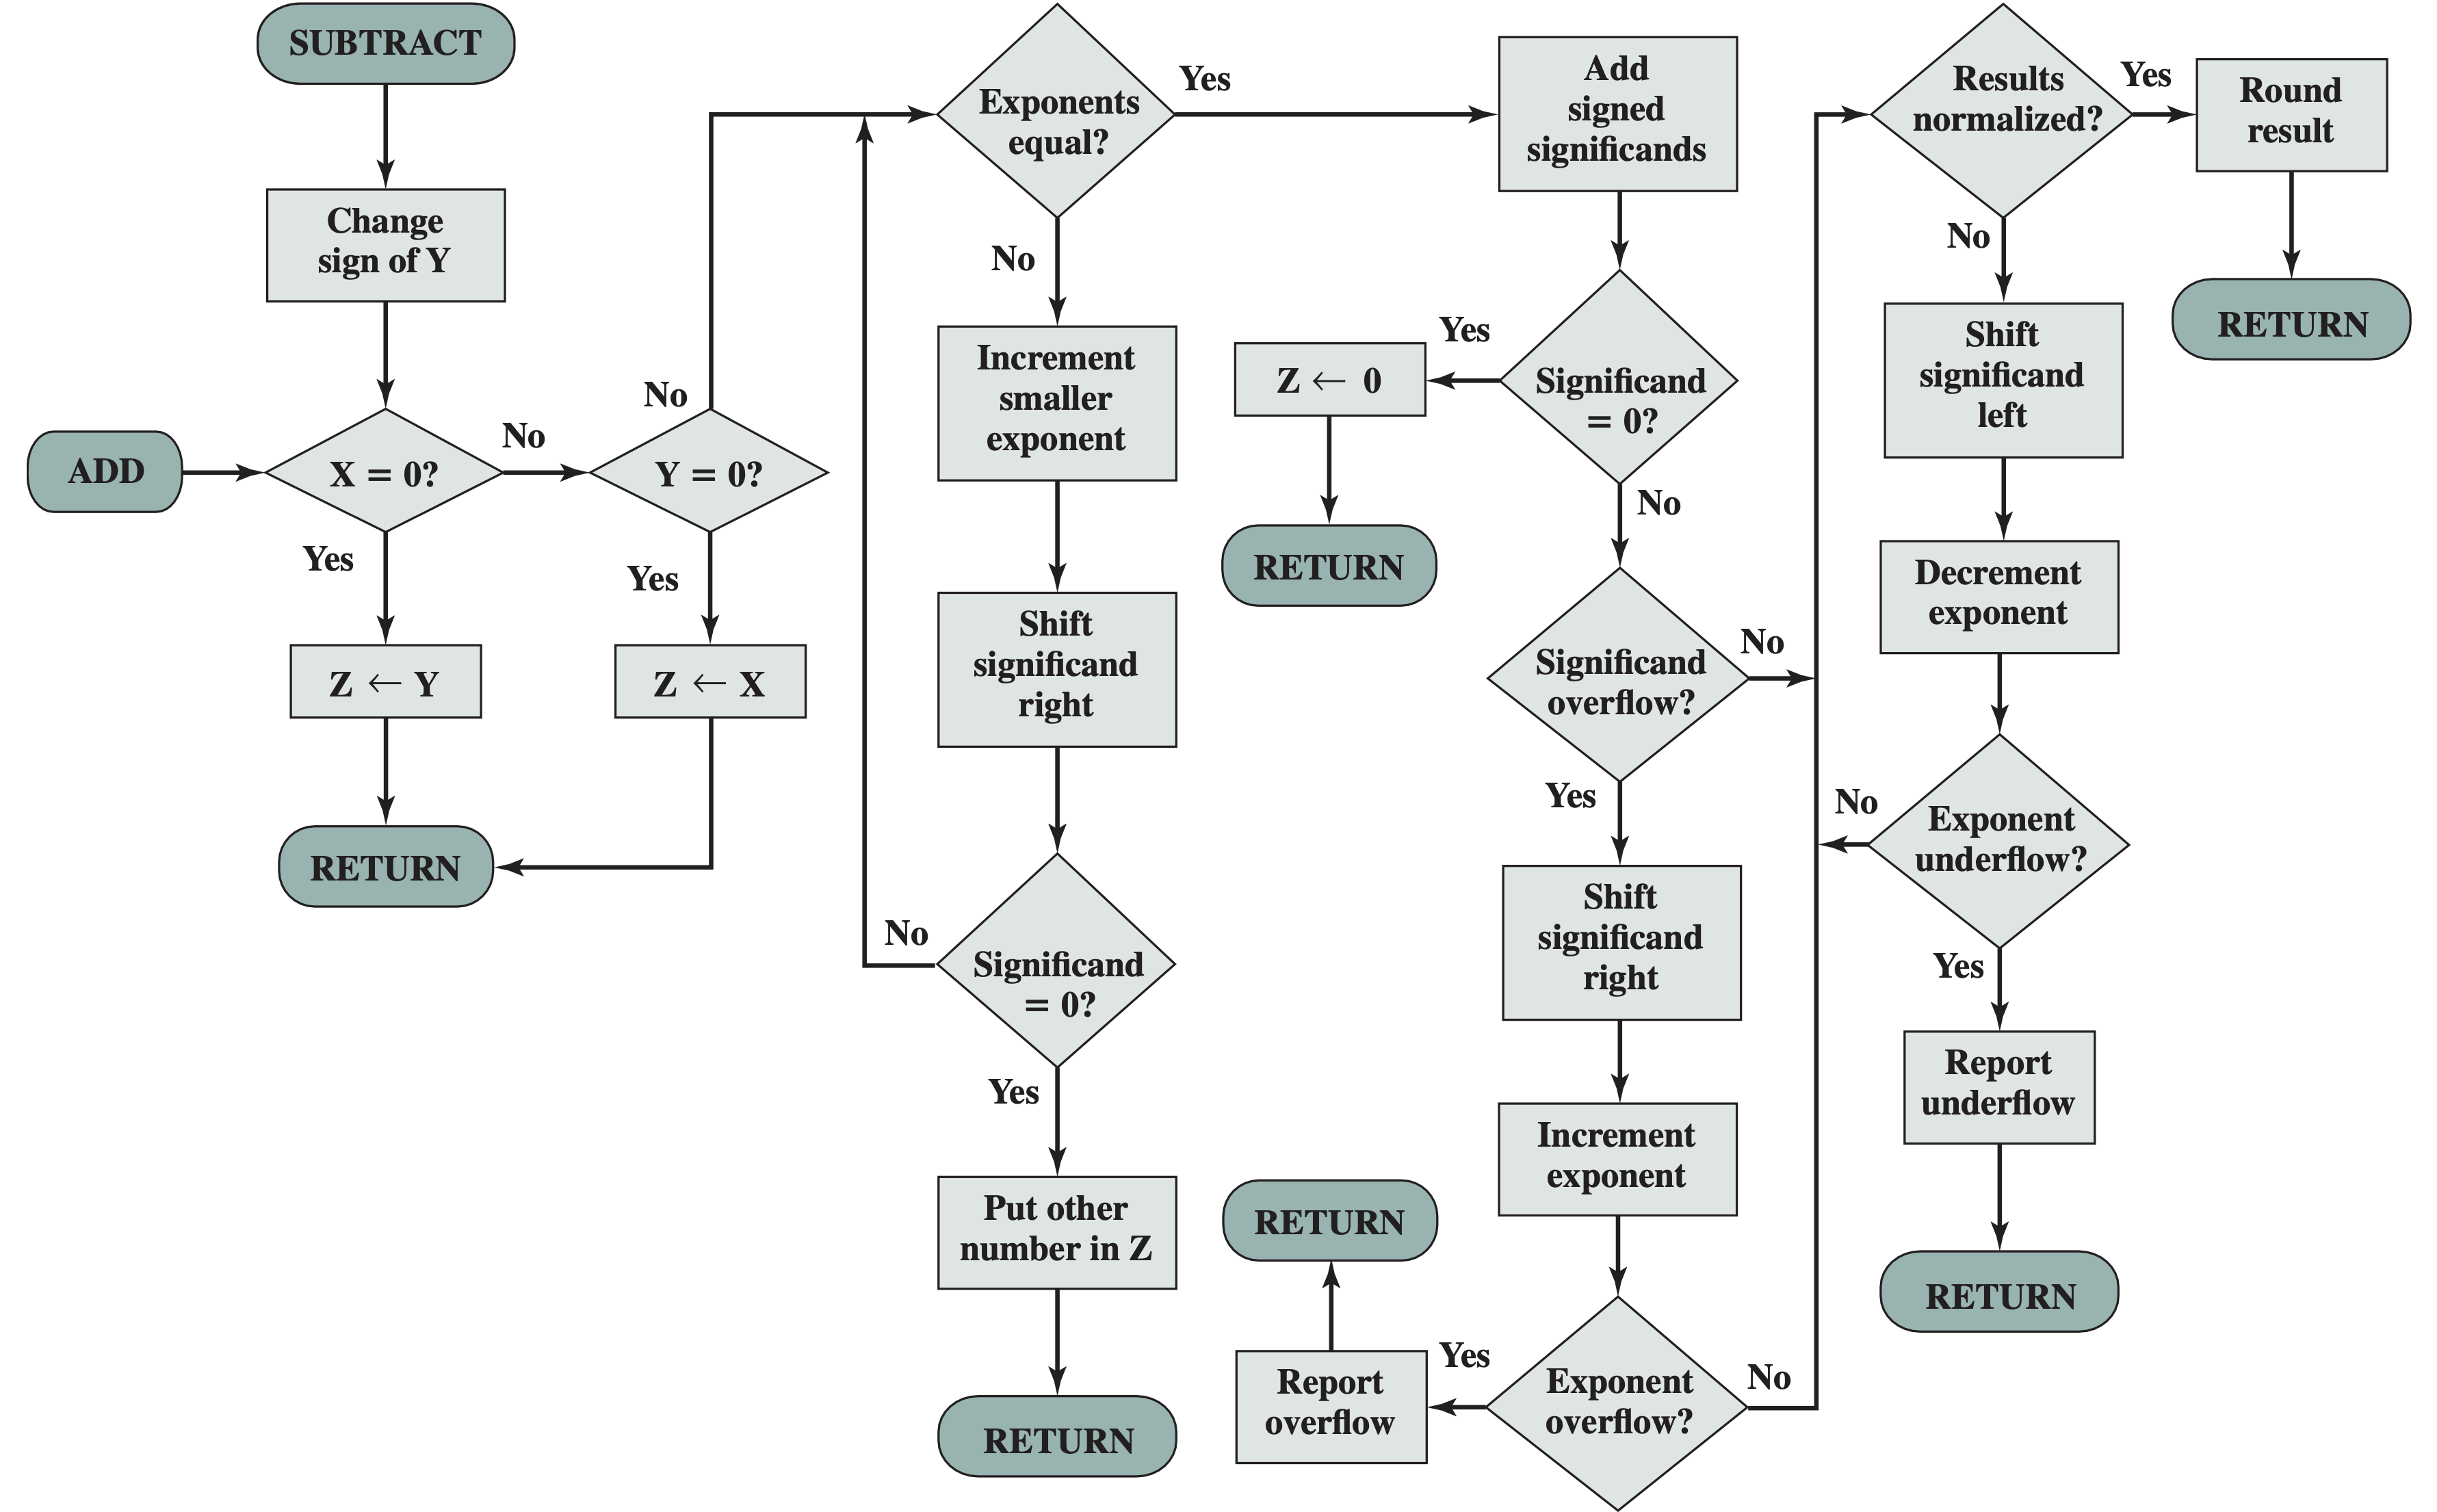
\includegraphics[scale=0.29]{chaps/number-representation/flt-add-sub-flow-chart.png}
\end{center}

\subsubsection{Multiplication}

Consider the multiplication illustrated in the equation:
\begin{equation*}
    \pm m_1\times 2^{\text{exp}_1} \times \pm m_2\times 2^{\text{exp}_2} =
    \pm m_1\times m_2\times 2^{\text{exp}_1 + \text{exp}_2}
\end{equation*}
where $\text{exp}$ is the real exponent value stored in Excess-$K$, whose bit pattern is
$\text{e} := \text{exp} + K$. To perform multiplication, the exponents are added, and the
significands are multiplied. The result is then normalised.

Consider the addition of the exponents' bit pattern, we have:
\begin{align*}
    \text{exp}_1 + \text{exp}_2 &= (\text{e}_1 - K) + (\text{e}_2 - K) \\
    \text{exp}_\text{sum} &= \text{e}_1 + \text{e}_2 - 2K \\
    \text{e}_\text{sum} - K &= \text{e}_1 + \text{e}_2 - 2K \\
    \text{e}_\text{sum} &= \text{e}_1 + \text{e}_2 - K
\end{align*}
Therefore, the bias $K$ is subtracted from the sum of the exponents' bit patterns.
Then, determine the sign of the result, and normalise and round the result.

\subsubsection{Division}

Division of floating-point numbers is similar to multiplication. It is defined by:
\begin{equation*}
    \frac{\pm m_1\times 2^{\text{exp}_1}}{\pm m_2\times 2^{\text{exp}_2}} =
    \pm \frac{m_1}{m_2}\times 2^{\text{exp}_1 - \text{exp}_2}
\end{equation*}

For the division of the exponents' bit patterns, we have:
\begin{align*}
    \text{exp}_1 - \text{exp}_2 &= (\text{e}_1 - K) - (\text{e}_2 - K) \\
    \text{exp}_\text{diff} &= \text{e}_1 - \text{e}_2 \\
    \text{e}_\text{diff} - K &= \text{e}_1 - \text{e}_2 \\
    \text{e}_\text{diff} &= \text{e}_1 - \text{e}_2 + K
\end{align*}
Therefore, the bit patterns of the exponents are subtracted, and the bias $K$ is added to the result.
Then, determine the sign of the result, and normalise and round the result.

Flowcharts showing floating-point multiplication and division are shown below.

\begin{center}
    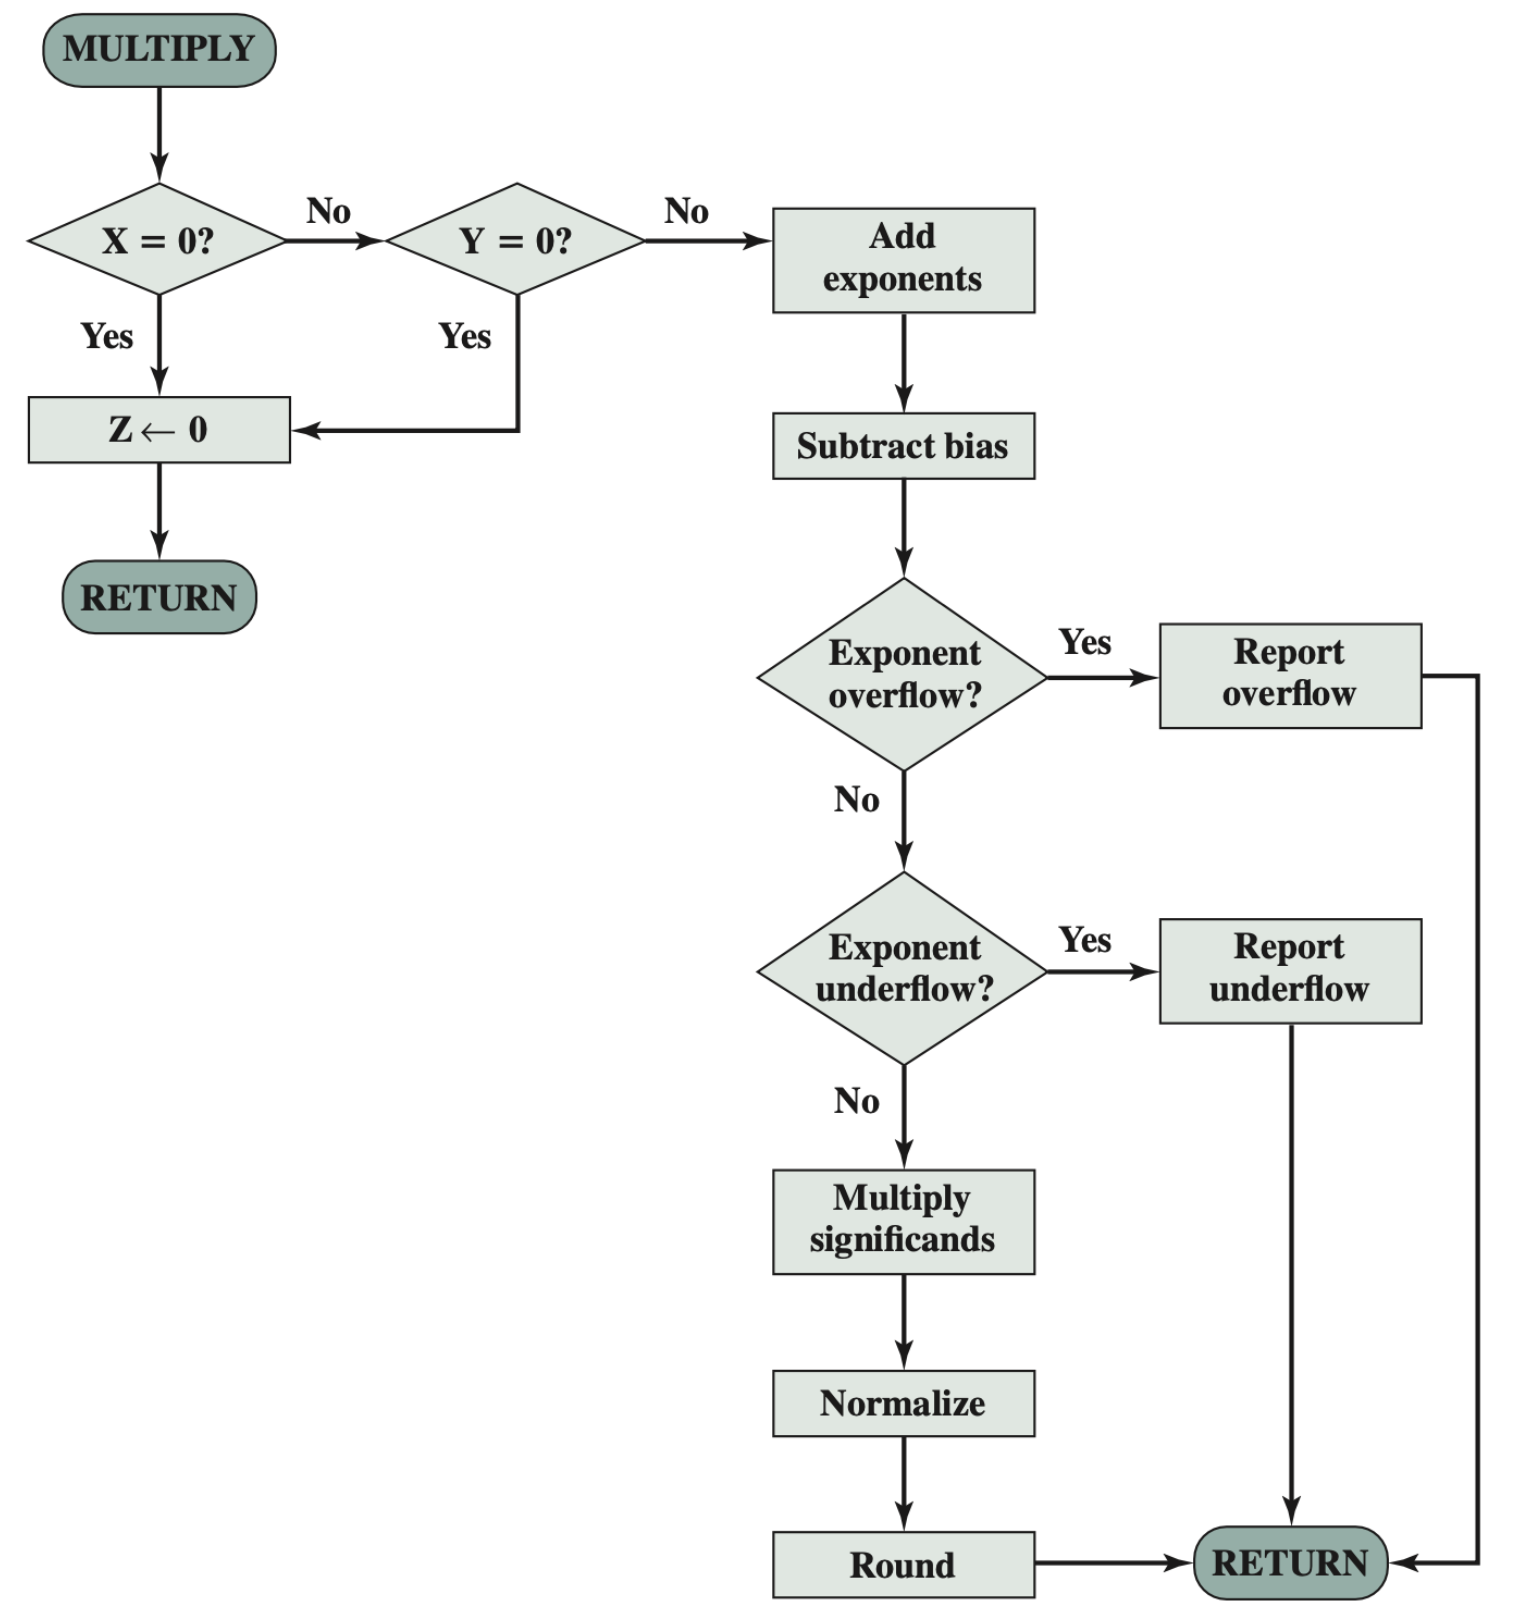
\includegraphics[width=0.45\linewidth]{chaps/number-representation/flt-multiply-flowchart.png}
    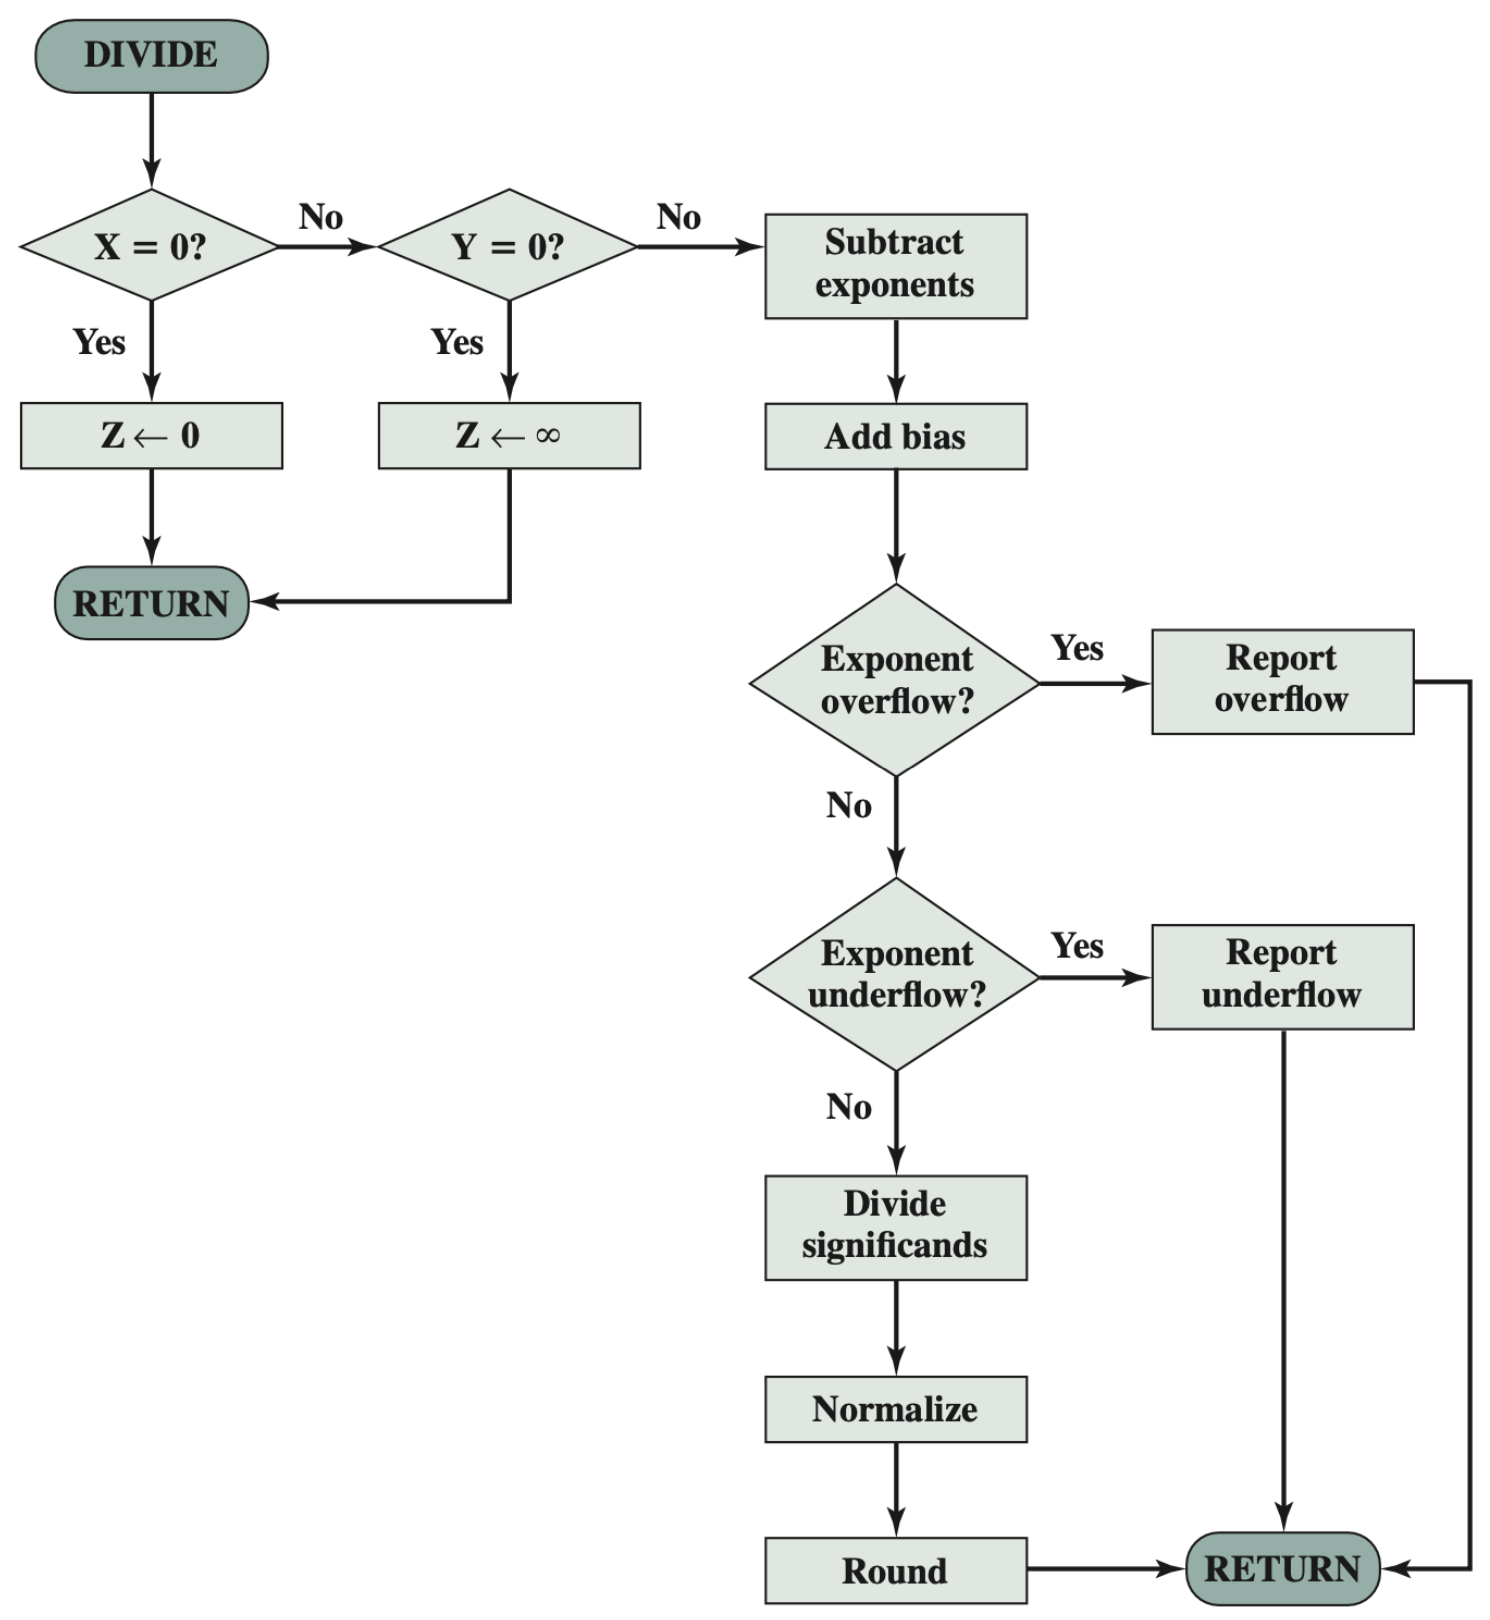
\includegraphics[width=0.45\linewidth]{chaps/number-representation/flt-divide-flowchart.png}
\end{center}

\subsubsection{Approximation of Floating-Point Arithmetic}

Floating-point numbers are prone to precision errors due to the following reasons:
\begin{itemize}
    \item Not all numbers can be represented precisely in binary,
        e.g. $0.2_{10} = $0.00110011\ldots$_2$.
    \item Round-off errors: some digits of the significand is lost to the left or right end
        of the significand when being shifted.
\end{itemize}

Due to errors, the Associative Law do not necessarily hold, especially when a very large number
is calculated with a very small number. In such cases, different orders of operations may yield
different results.

Different approaches for rounding a floating-point number include
\begin{enumerate*}
    \item round to nearest,
    \item round towards zero,
    \item round towards $\pm\infty$.
\end{enumerate*}